\documentclass[12pt]{beamer}
%\documentclass[20pt,handout]{beamer}
\usetheme{Darmstadt}
\usepackage{graphicx}
%\usepackage[german]{babel}
\usepackage[T1]{fontenc}
\usepackage[utf8]{inputenc}
\usepackage{tikz}
\setbeamertemplate{footline}[frame number]
\usepackage{multicol}

% fix appendix

\usepackage{etoolbox}
\makeatletter
\patchcmd{\beamer@part}{\setcounter{subsection}{0}}{}{}
\makeatother

% code listing stuff

\makeatletter
\newcommand{\miniscule}{\@setfontsize\miniscule{5}{6}}% \tiny: 6/7
\makeatother

\usepackage{listings}
\usepackage{color}
\definecolor{lightgray}{rgb}{.9,.9,.9}
\definecolor{darkgray}{rgb}{.4,.4,.4}
\definecolor{purple}{rgb}{0.65, 0.12, 0.82}

\lstdefinelanguage{JavaScript}{
  keywords={typeof, new, true, false, catch, function, return, null, catch, switch, var, if, in, while, do, else, case, break},
  keywordstyle=\color{blue}\bfseries,
  ndkeywords={class, export, boolean, throw, implements, import, this},
  ndkeywordstyle=\color{darkgray}\bfseries,
  identifierstyle=\color{black},
  sensitive=false,
  comment=[l]{//},
  morecomment=[s]{/*}{*/},
  commentstyle=\color{purple}\ttfamily,
  stringstyle=\color{red}\ttfamily,
  morestring=[b]',
  morestring=[b]"
}

\lstset{
   language=JavaScript,
   frame=single,
   backgroundcolor=\color{lightgray},
   extendedchars=true,
   basicstyle=\tiny\ttfamily,
   showstringspaces=false,
   showspaces=false,
   numbers=left,
   numberstyle=\tiny,
   numbersep=9pt,
   tabsize=2,
   breaklines=true,
   showtabs=false,
   captionpos=b
}



\title{\small Datenschutz \& Datensicherheit von \\ \huge WebRTC}
\author{Stephan Thamm}
\date{26.06.2015}

\begin{document}
\maketitle

\frame{\tableofcontents[sections={1-4}]}


\section{Was ist WebRTC?}
\subsection{} 

\begin{frame}
  \frametitle{Was ist WebRTC?}
  \begin{itemize}
    \item<2-> \textbf{Web} \textbf{R}eal \textbf{T}ime \textbf{C}ommunication
    \item<3-> getUserMedia()
    \item<4-> PeerConnection
    \item<5-> DataChannel
  \end{itemize}
\end{frame}

\begin{frame}
  \frametitle{Palava}
  \includegraphics<1>[height=0.7\textheight]{img/palava_1.jpg}
  \includegraphics<2>[height=0.7\textheight]{img/palava_2.jpg}
  \includegraphics<3>[height=0.7\textheight]{img/palava_3.jpg}
  \\ \hfill \tiny https://palava.tv
\end{frame}

\begin{frame}
  \frametitle{Sharefest}
  \centerline{
\includegraphics[width=0.5\textwidth]{img/sharefest.png}}
  \centerline{\tiny https://sharefest.me}
\end{frame}

\begin{frame}
  \frametitle{Cube Slam}
  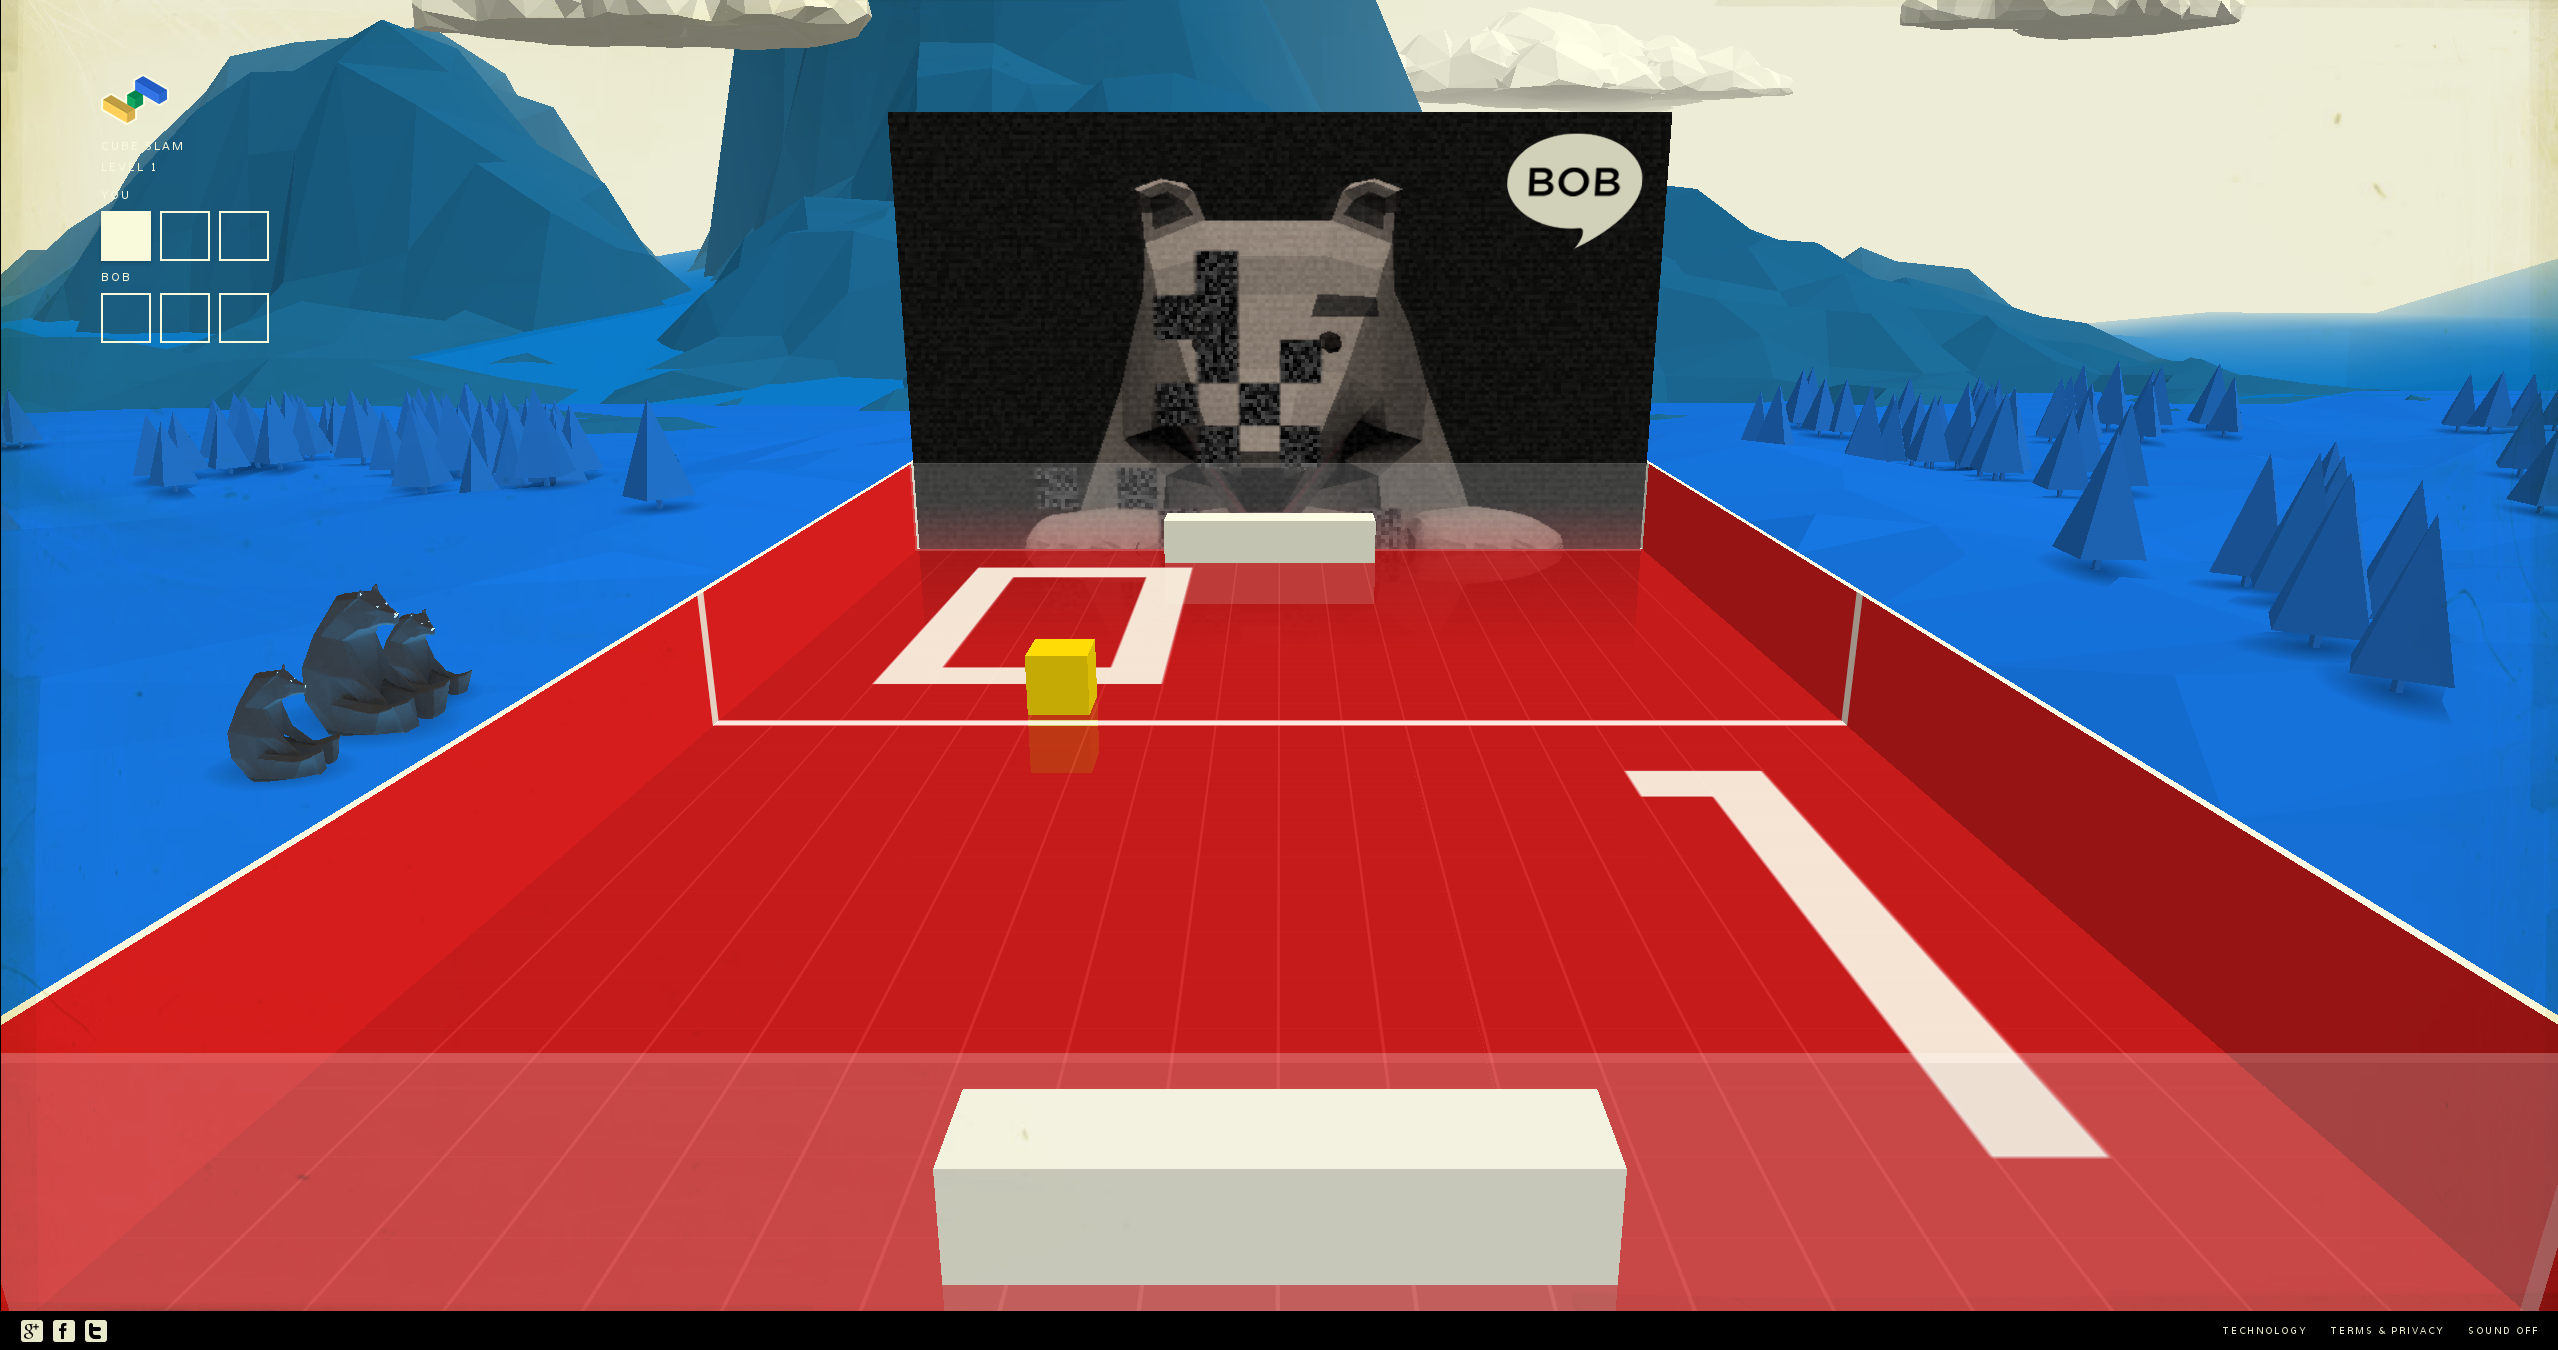
\includegraphics[height=0.7\textheight]{img/cube_slam.png} \\
  \hfill \tiny https://www.cubeslam.com
\end{frame}

\begin{frame}
  \frametitle{Standardisierung}
  \begin{itemize}
    \item<2-> 2011 von Google initiiert
    \item<3-> Work in Progress
    \item<4-> WebRTC Gruppe in W3C
    \item<5-> RTCWEB Gruppe in IETF
    \item<6-> ORTC/WebRTC 1.1
  \end{itemize}
\end{frame}

\begin{frame}
  \frametitle{Verbreitung}
  \pause
  \centerline{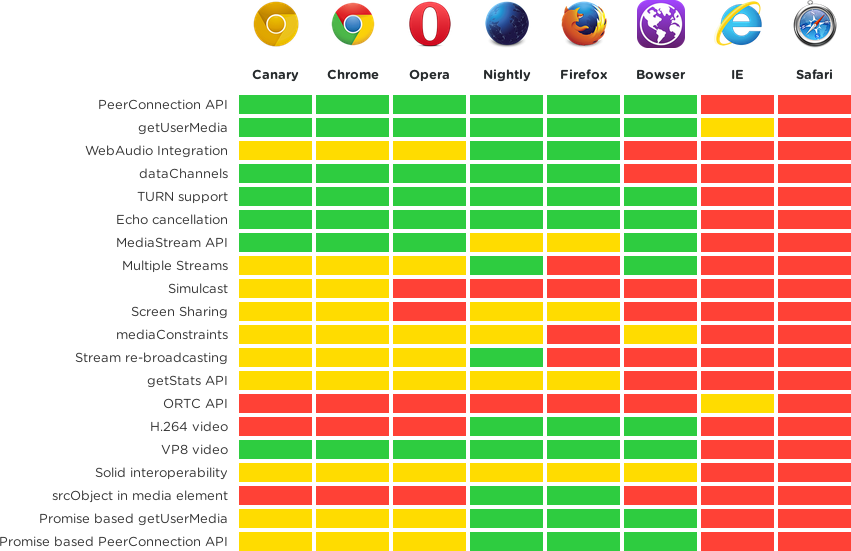
\includegraphics[height=0.7\textheight]{img/webrtc_ready.png}}
  \hfill \tiny http://iswebrtcreadyyet.com/ \\
  \hfill \tiny Stand 10.06.2015
\end{frame}


\section{Anwendungssicht}
\subsection{} 

\begin{frame}
  \frametitle{getUserMedia()}
  \pause
  \lstinputlisting{examples/gum.js}
\end{frame}

\begin{frame}
  \frametitle{Kamerazugriff}
  \pause
  \centerline{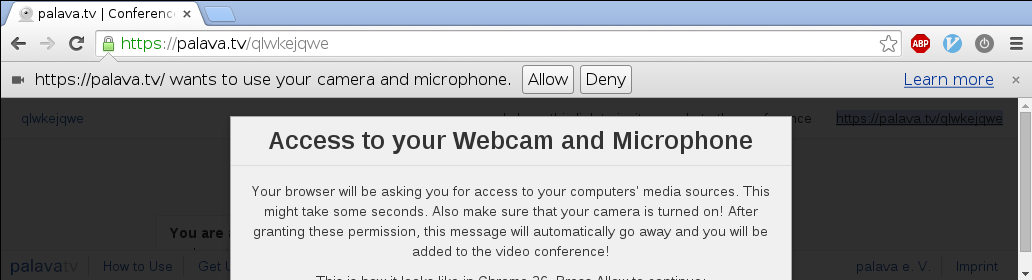
\includegraphics[width=0.7\textwidth]{img/access_chrome.png}}
  %\hfill \tiny Chrome
  \vspace{15pt}
  \centerline{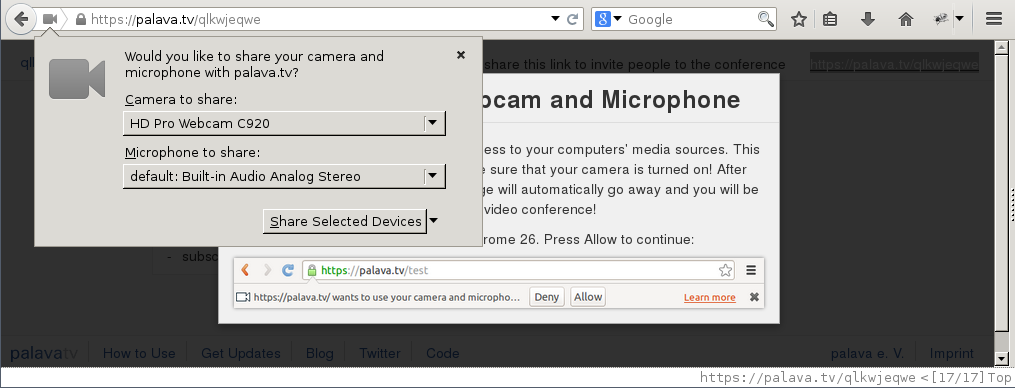
\includegraphics[width=0.7\textwidth]{img/access_firefox.png}}
  %\hfill \tiny Firefox
\end{frame}

\begin{frame}
  \frametitle{Peer to Peer}
  \begin{itemize}
    \item Holding ...
    \item ... places
  \end{itemize}
\end{frame}

\begin{frame}
  \frametitle{Multipoint Control Unit (MCU)}
  \begin{itemize}
    \item Holding ...
    \item ... places
  \end{itemize}
\end{frame}

\begin{frame}
  \frametitle{Signaling}
  \begin{itemize}
    \item Holding ...
    \item ... places
  \end{itemize}
\end{frame}

\begin{frame}
  \frametitle{palava-client}
  \pause
  \lstinputlisting{examples/palava.js}
\end{frame}


\section{Verbindungsaufgbau}
\subsection{} 

\begin{frame}
  \frametitle{Session Description Protocol (SDP)}
  \pause
  \begin{multicols}{2}
    \lstinputlisting[language={},numbers=none,basicstyle=\miniscule\ttfamily]{examples/sdp.txt}
  \end{multicols}
\end{frame}

\begin{frame}
  \frametitle{Ablauf}
  \begin{itemize}
    \item Holding ...
    \item ... places
  \end{itemize}
\end{frame}

\begin{frame}
  \frametitle{Interactive Connectivity Establishment (ICE)}
  \pause
  \lstinputlisting[language={},numbers=none,firstline=34,lastline=35,basicstyle=\tiny\ttfamily]{examples/sdp.txt}
  \hfill \tiny Auszug Offer/Answer
  \vspace{15pt}
  \pause
  \lstinputlisting[language={},numbers=none,basicstyle=\tiny\ttfamily,firstline=1,lastline=1]{examples/ice_trickle.txt}
  \lstinputlisting[language={},numbers=none,basicstyle=\tiny\ttfamily,firstline=2,lastline=2]{examples/ice_trickle.txt}
  \hfill \tiny ICE Trickling
\end{frame}

\begin{frame}
  \frametitle{Probleme}
  \begin{itemize}
    \item<2-> Peer erhält alle IP Adressen
    \item<3-> Fingerprinting
    \item<4-> Umgehung von VPNs
  \end{itemize}
\end{frame}


\section{On the Wire}
\subsection{} 

\begin{frame}
  \frametitle{Protokolle}
  \centerline{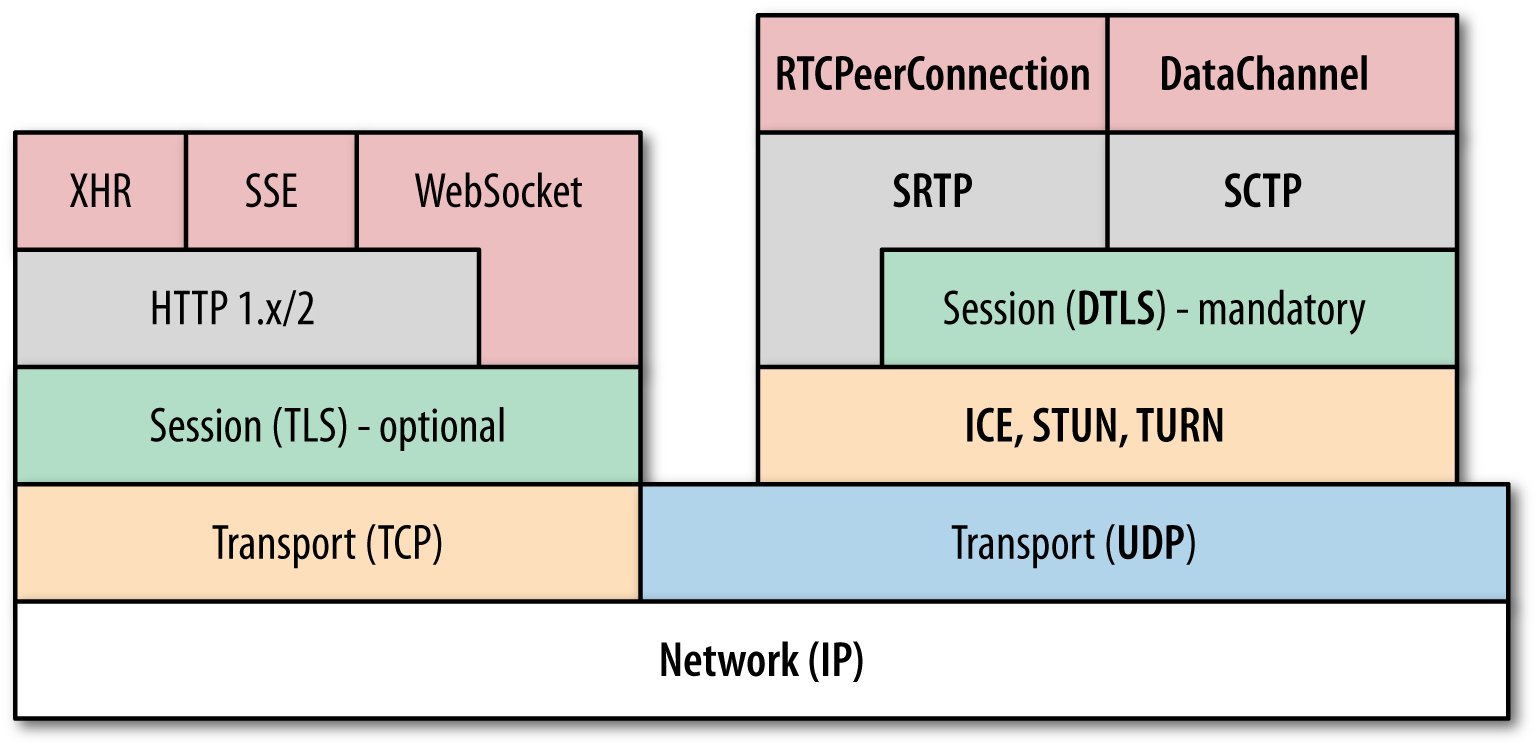
\includegraphics[width=0.7\textwidth]{img/stack_oreilly.png}}
\end{frame}

\begin{frame}
  \frametitle{Signaling}
  \centerline{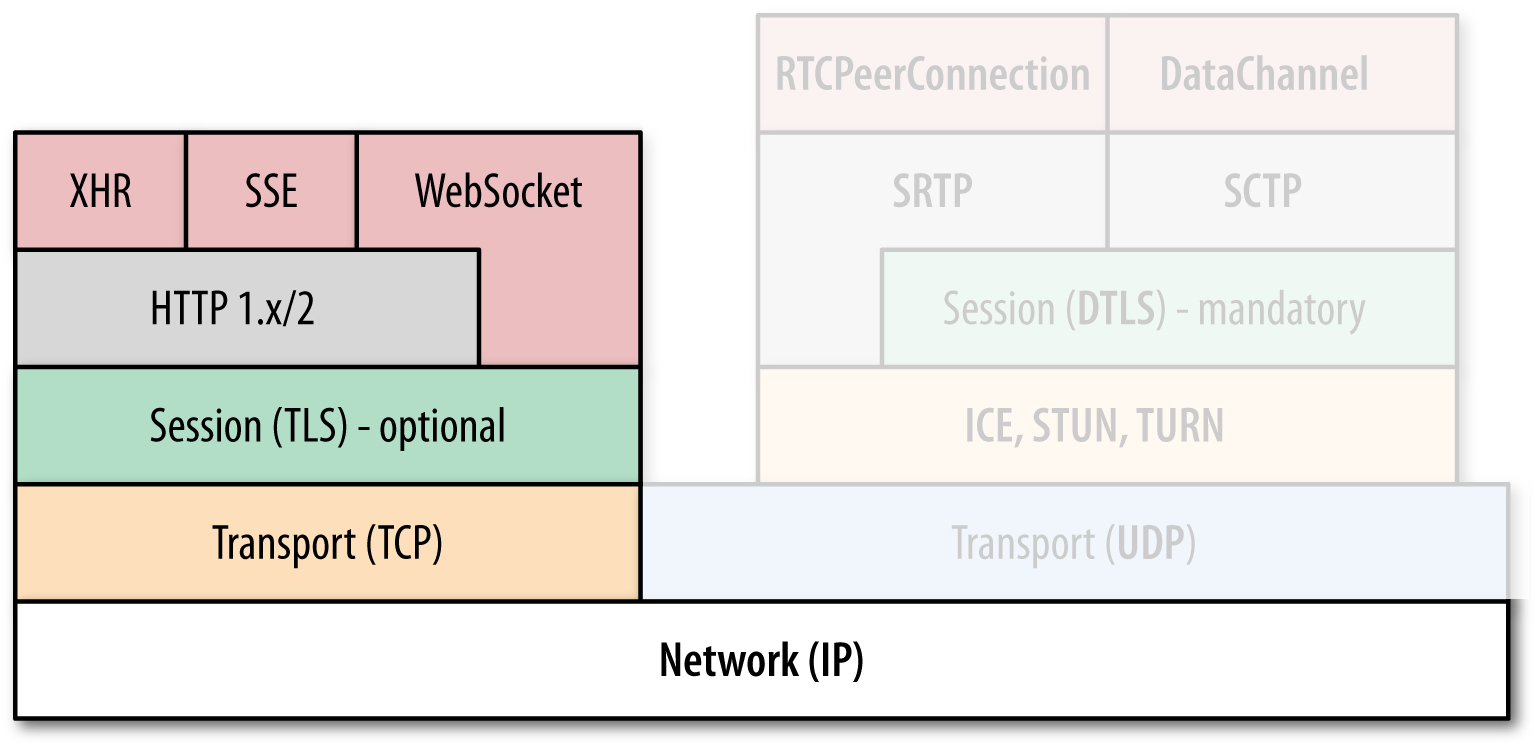
\includegraphics[width=0.7\textwidth]{img/stack_oreilly_signaling.png}}
\end{frame}

\begin{frame}
  \frametitle{PeerConnection}
  \centerline{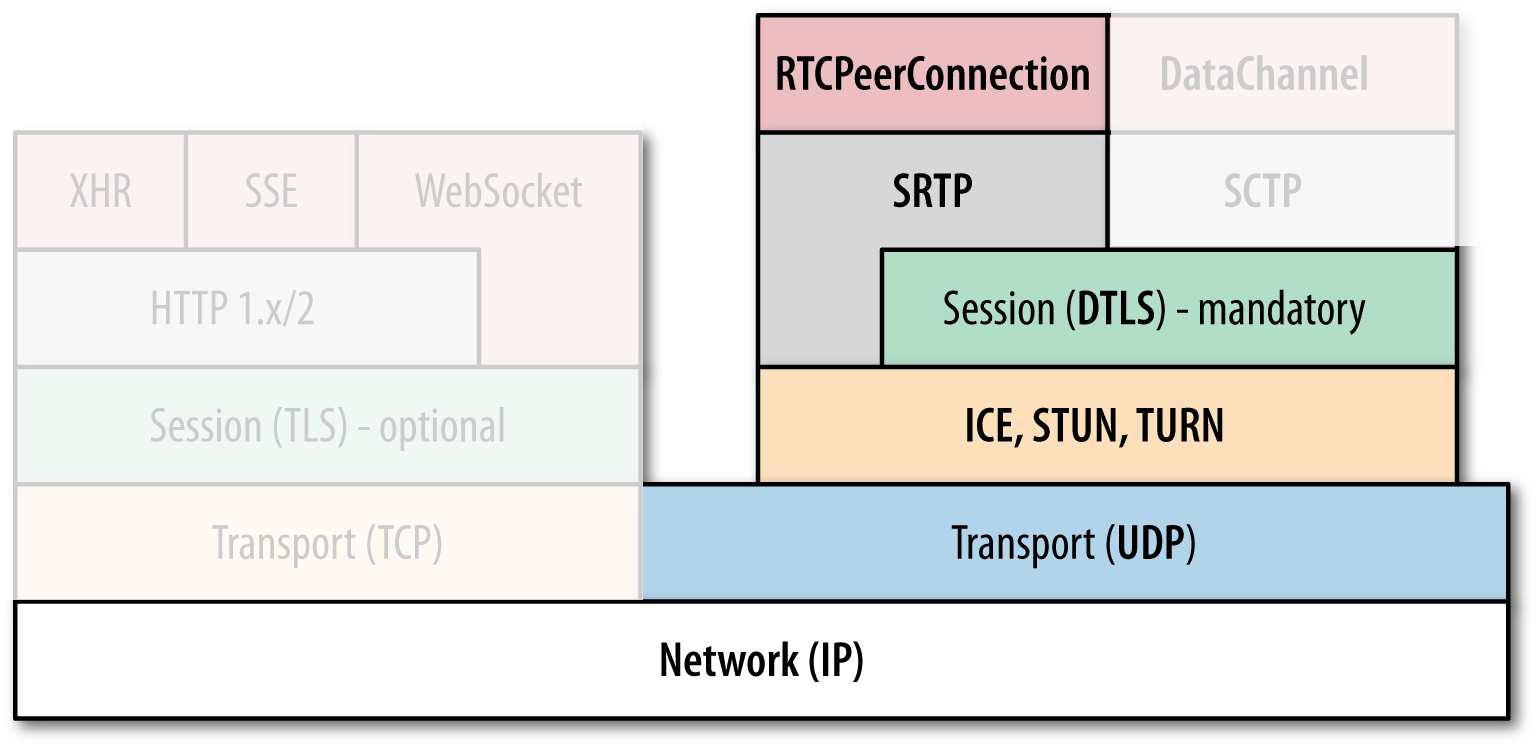
\includegraphics[width=0.7\textwidth]{img/stack_oreilly_pc.png}}
\end{frame}

\begin{frame}
  \frametitle{Schlüsselaustausch}
  \pause
  \lstinputlisting[language={},numbers=none,firstline=9,lastline=9,basicstyle=\small\ttfamily]{examples/sdp.txt}
  \hfill \tiny SDES, Auszug Offer/Answer
  \vspace{15pt} \\
  \pause
  \lstinputlisting[language={},numbers=none,firstline=7,lastline=7,basicstyle=\small\ttfamily]{examples/sdp.txt}
  \hfill \tiny DTLS-SRTP, Auszug Offer/Answer
\end{frame}

\begin{frame}
  \frametitle{DataChannel}
  \centerline{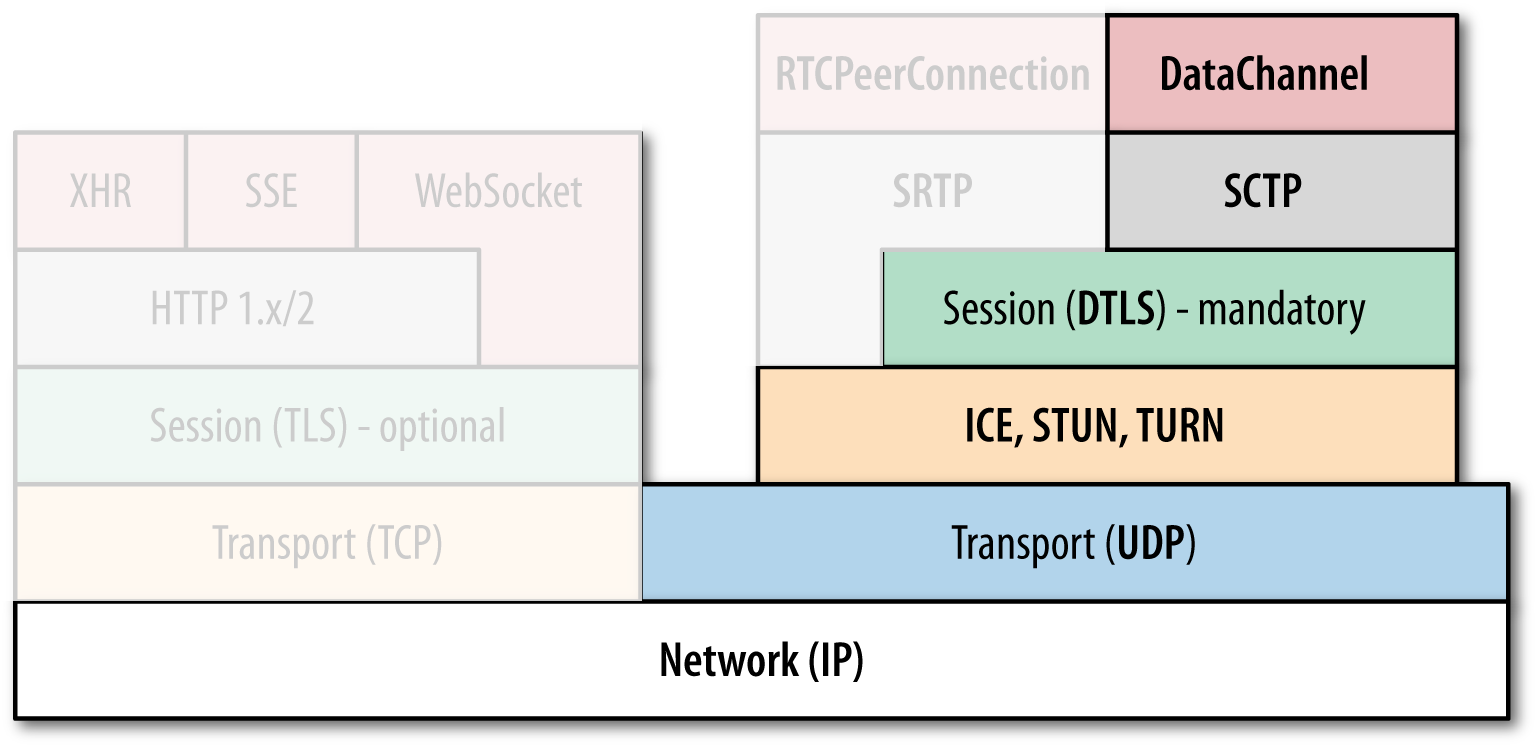
\includegraphics[width=0.7\textwidth]{img/stack_oreilly_datachannels.png}}
\end{frame}

\begin{frame}
  \frametitle{Man in the Middle - Signaling}
  \begin{itemize}
    \item Holding ...
    \item ... places
  \end{itemize}
\end{frame}

\begin{frame}
  \frametitle{Man in the Middle - Website}
  \begin{itemize}
    \item Holding ...
    \item ... places
  \end{itemize}
\end{frame}


\section{Fazit}
\subsection{}

\begin{frame}
  \frametitle{Sicherheitskritische Aspekte}
  \begin{itemize}
    \item Kamera- und Mikrofonzugriff
    \item Peers erhalten alle IP Adressen
    \item Umgehung von VPNs
    \item Fingerprinting
    \item Authentifizierung der Peers
    \item Vertrauen in Website-Code
  \end{itemize}
\end{frame}

\end{document}
